\documentclass{article}
\usepackage[utf8]{inputenc}

\usepackage[T2A]{fontenc}
\usepackage[utf8]{inputenc}
\usepackage[russian]{babel}

\usepackage{amsmath}
\usepackage{graphicx}

\title{Вычислительная техника}
\author{Лисид Лаконский}
\date{October 2022}

\begin{document}

\maketitle
\tableofcontents
\pagebreak

\section{Вычислительная техника - 17.10.2022}

\subsection{Шифраторы}

\begin{flushleft}

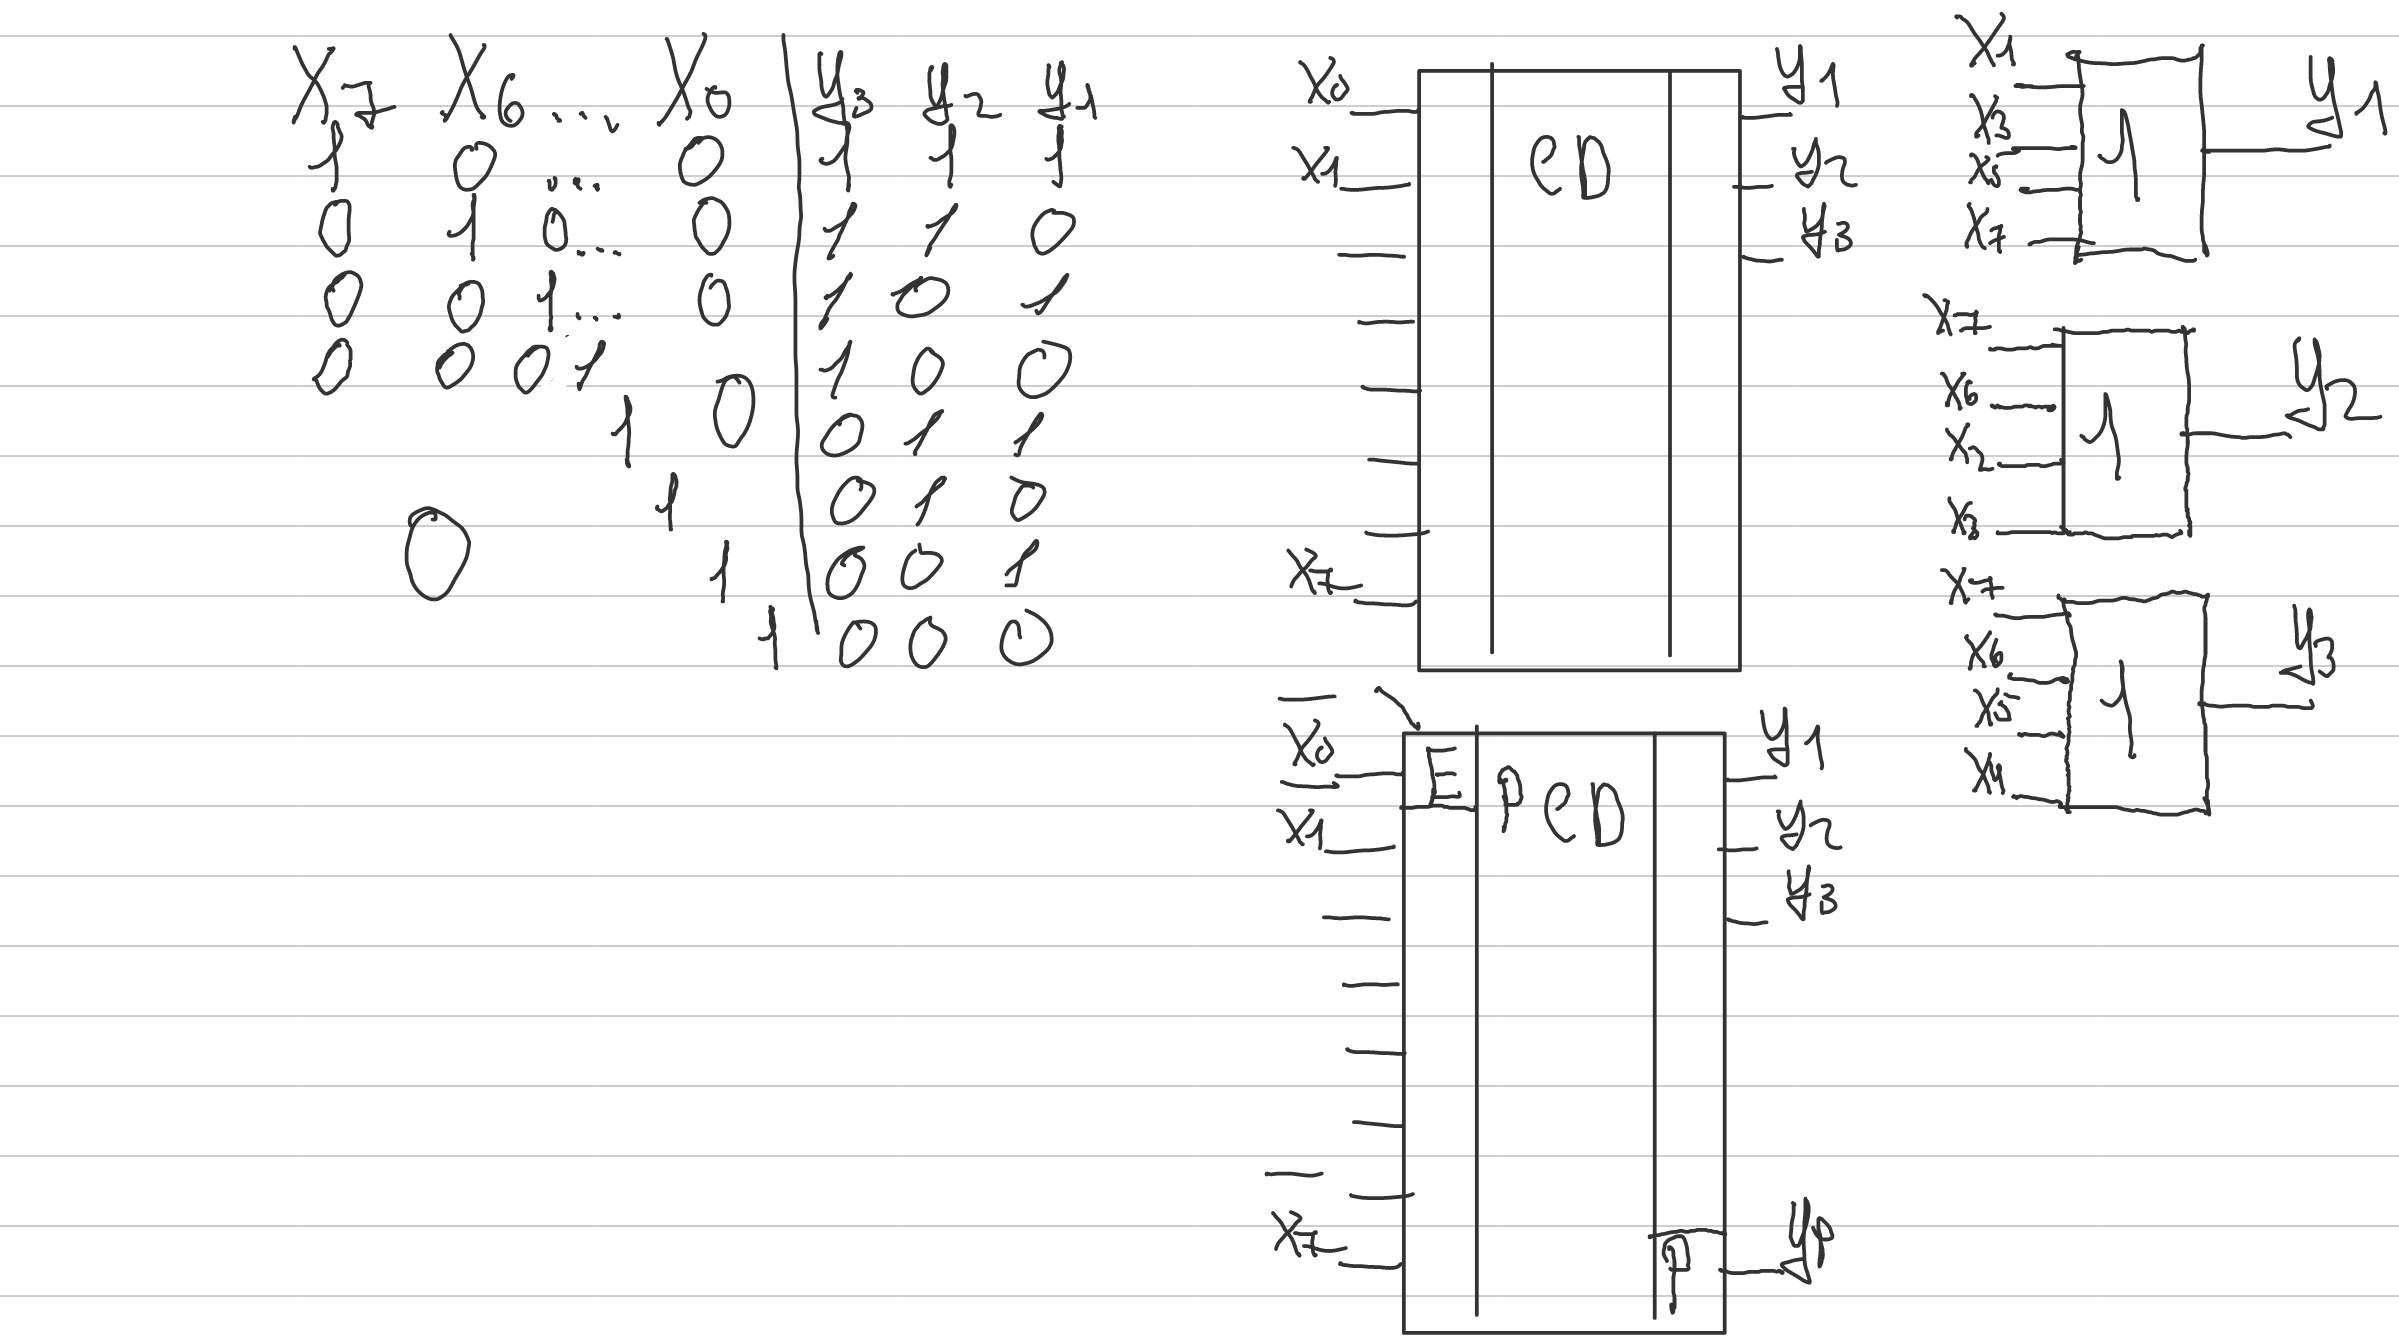
\includegraphics[width=\textwidth]{assets/coder.png}

\subsubsection{Устранение неоднозначности}

Устранять неоднозначность можно с помощью приоритетного шифратора - дополнительный выход $p$ - выход признака невозбуждения: 0 - возбужден хотя бы один из входов, 1 - в противном случае, дополнительный вход $E$.

\subsection{Дешифраторы}

\subsubsection{Линейные дешифраторы}

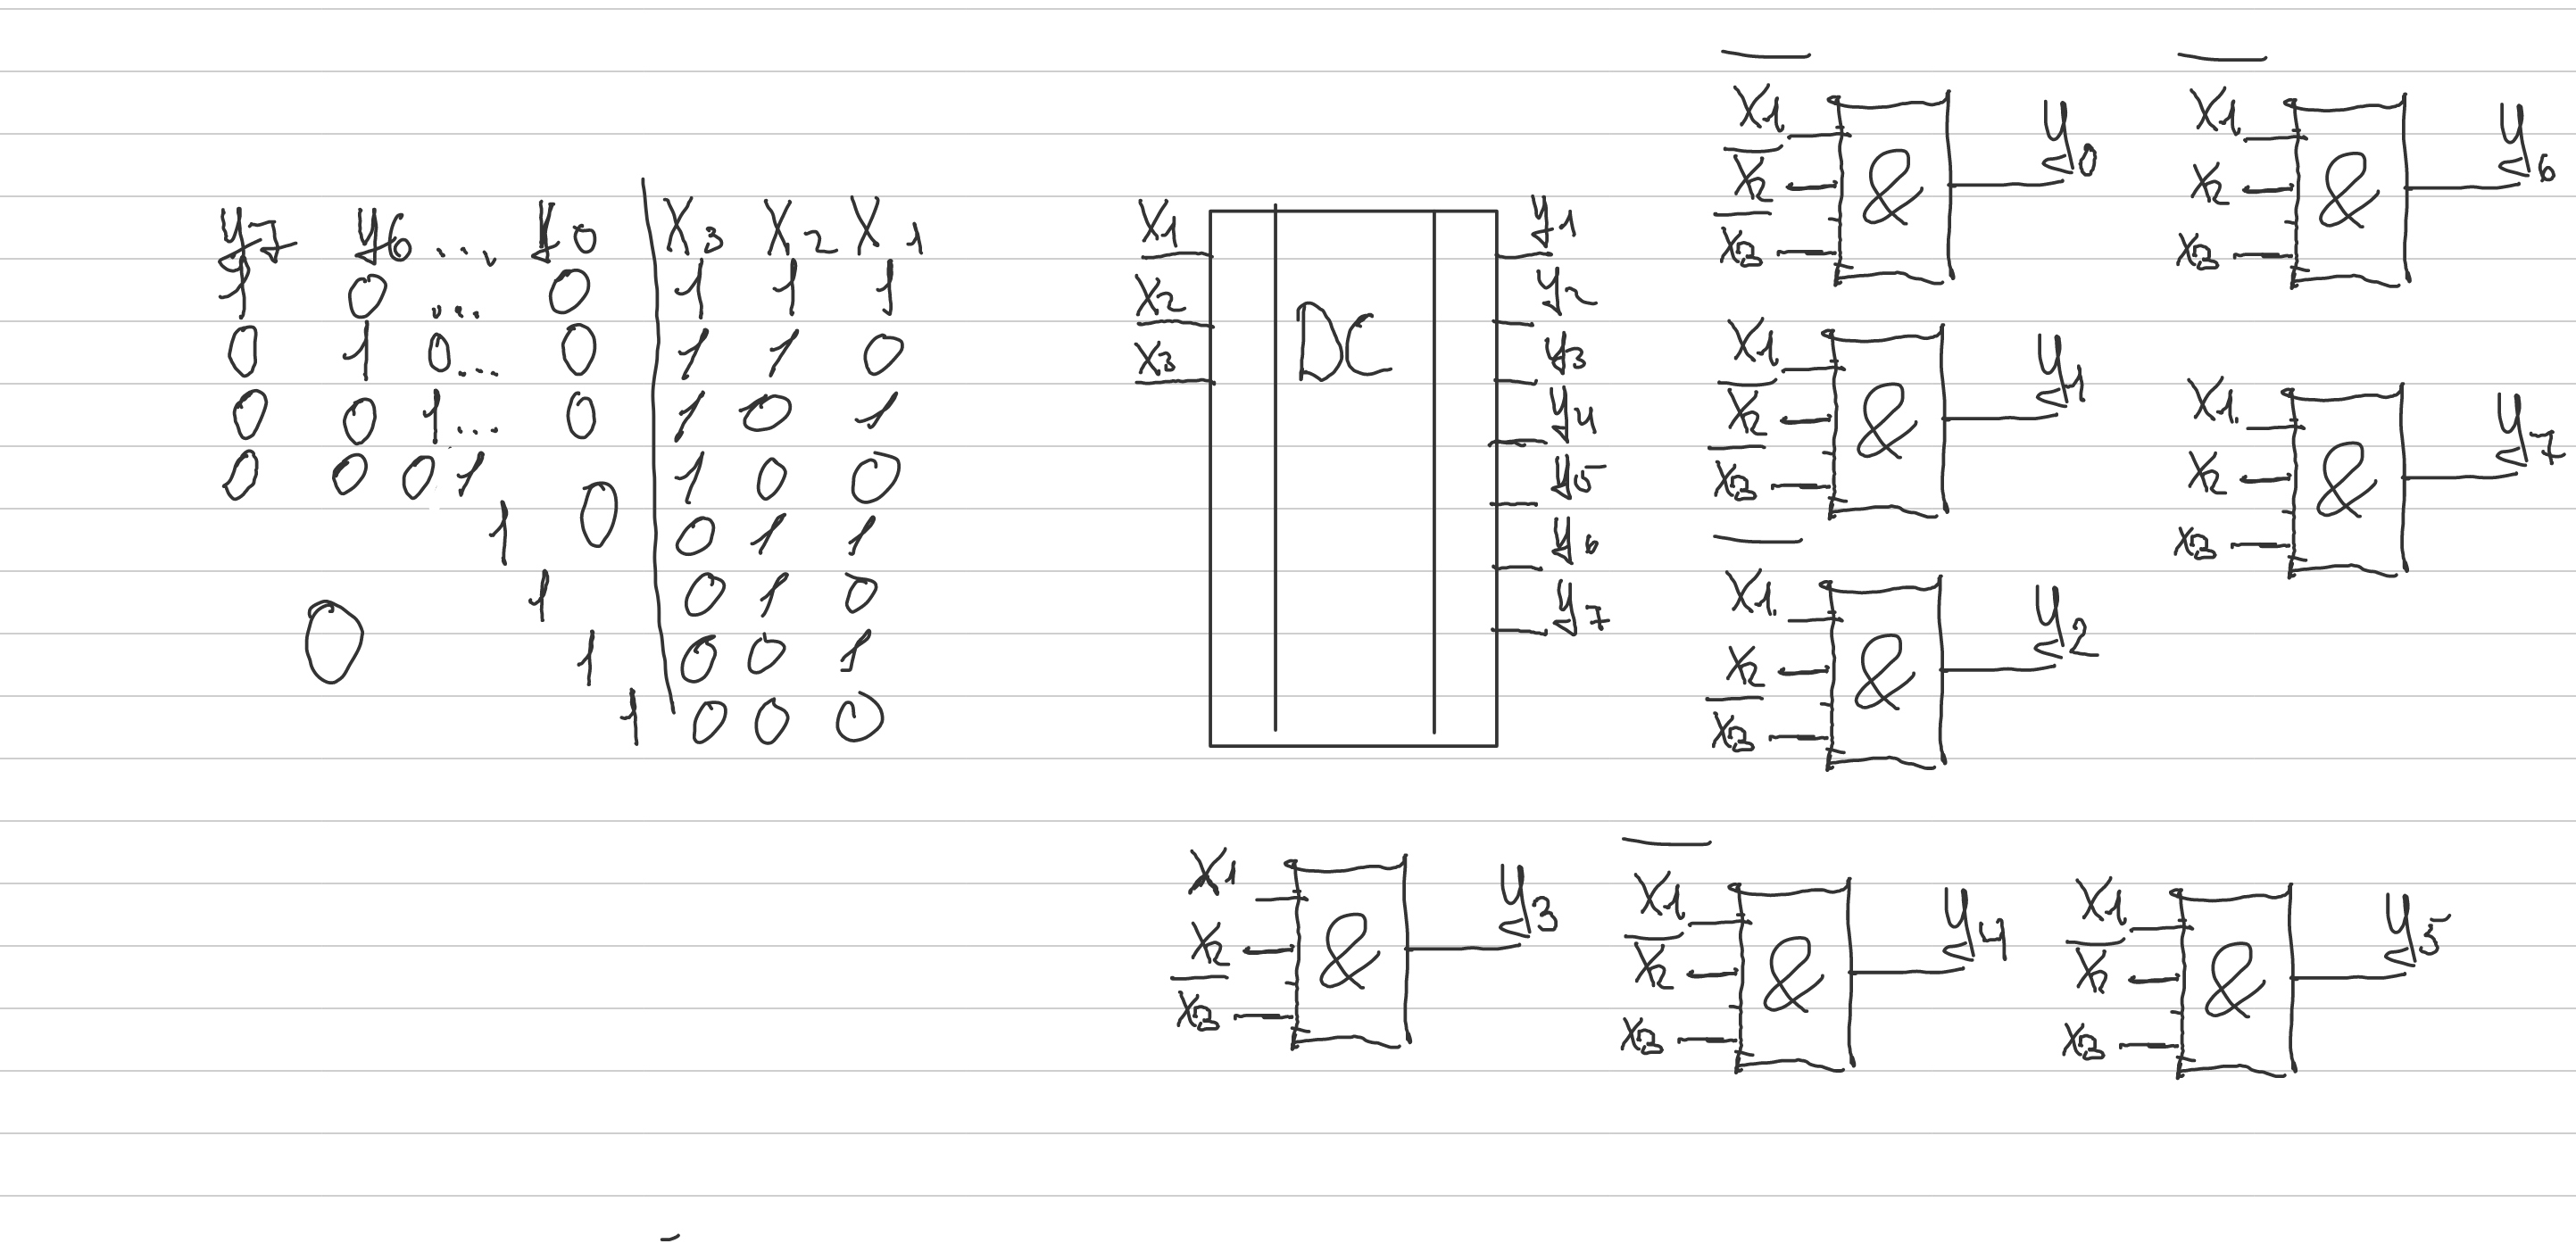
\includegraphics[width=\textwidth]{assets/decoder.png}

\hfill

Ниже приведено обозначение микросхемы К155ИД4

\hfill

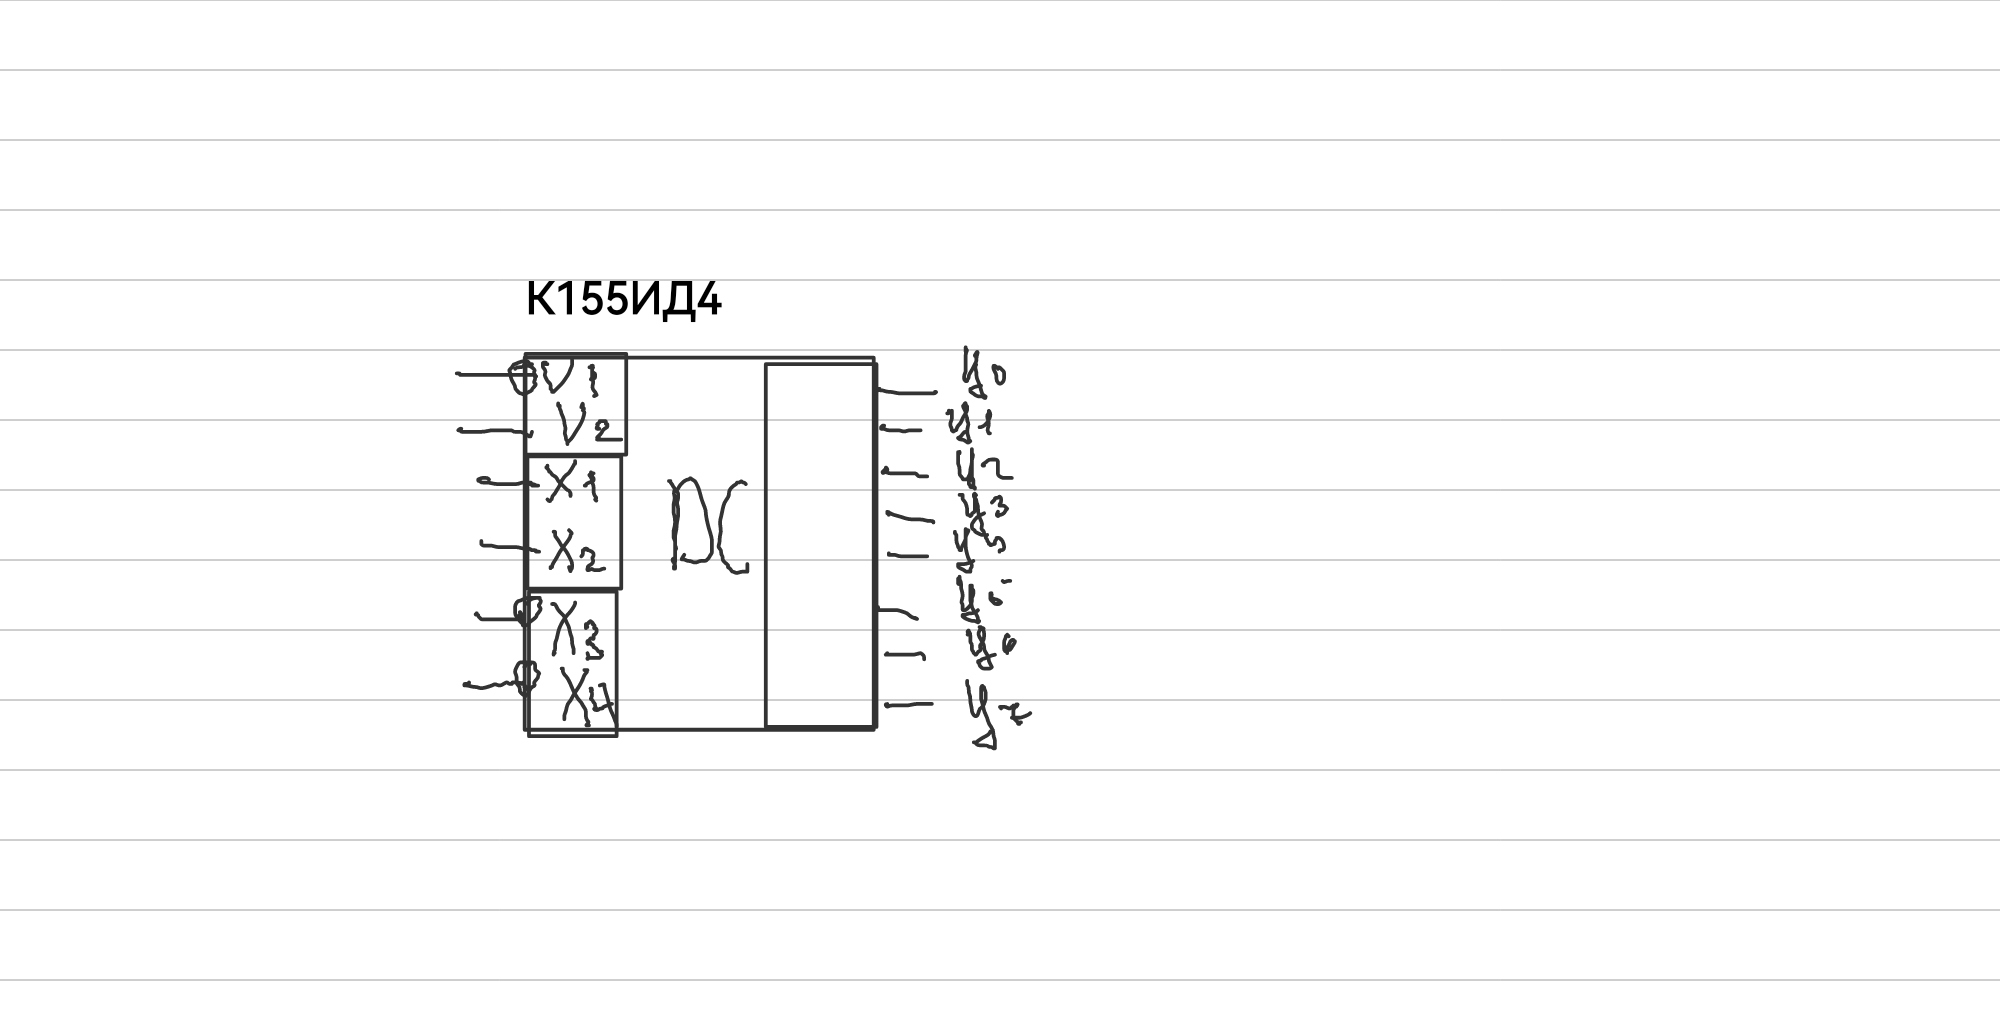
\includegraphics[width=\textwidth]{assets/k155id4.png}

Существуют также пирамидальные, каскадные дешифраторы.

\subsubsection{Каскадный дешифратор}

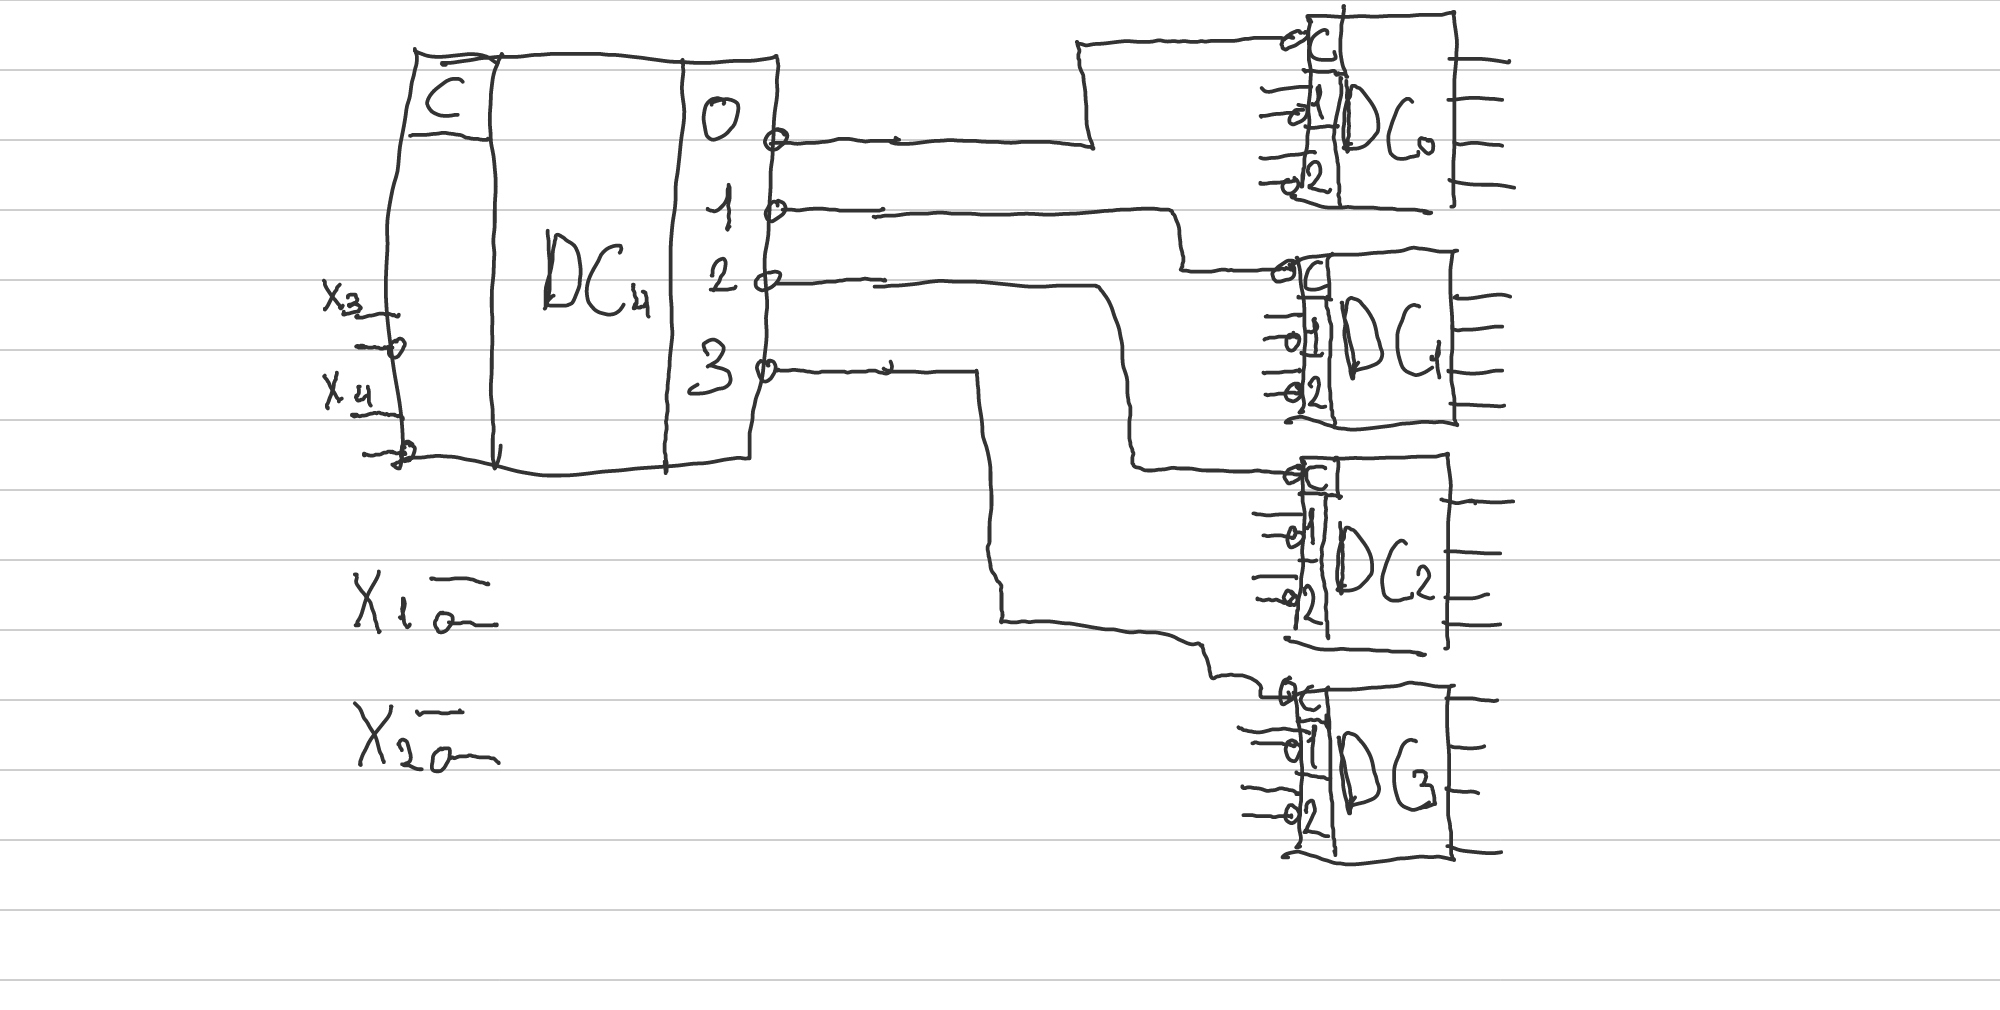
\includegraphics[width=\textwidth]{assets/cascade.png}

\subsection{Мультплексор}

Мультиплексор обеспечивает коммутацию на вход одного из входных сигналов.

Формула:

$y = \overline{x_3}\overline{x_2}\overline{x_1}D_0 + \overline{x_3}\overline{x_2}x_1D_1 + \overline{x_3}x_2\overline{x_1}D_2 + ... + x_3x_2x_1D_7$

\hfill

В формулу может быть добавлен управляющий сигнал:

$y = \overline{x_3}\overline{x_2}\overline{x_1}D_0\overline{v} + \overline{x_3}\overline{x_2}x_1D_1\overline{v} + \overline{x_3}x_2\overline{x_1}D_2\overline{v} + ... + x_3x_2x_1D_7\overline{v}$

\subsubsection{Схема}

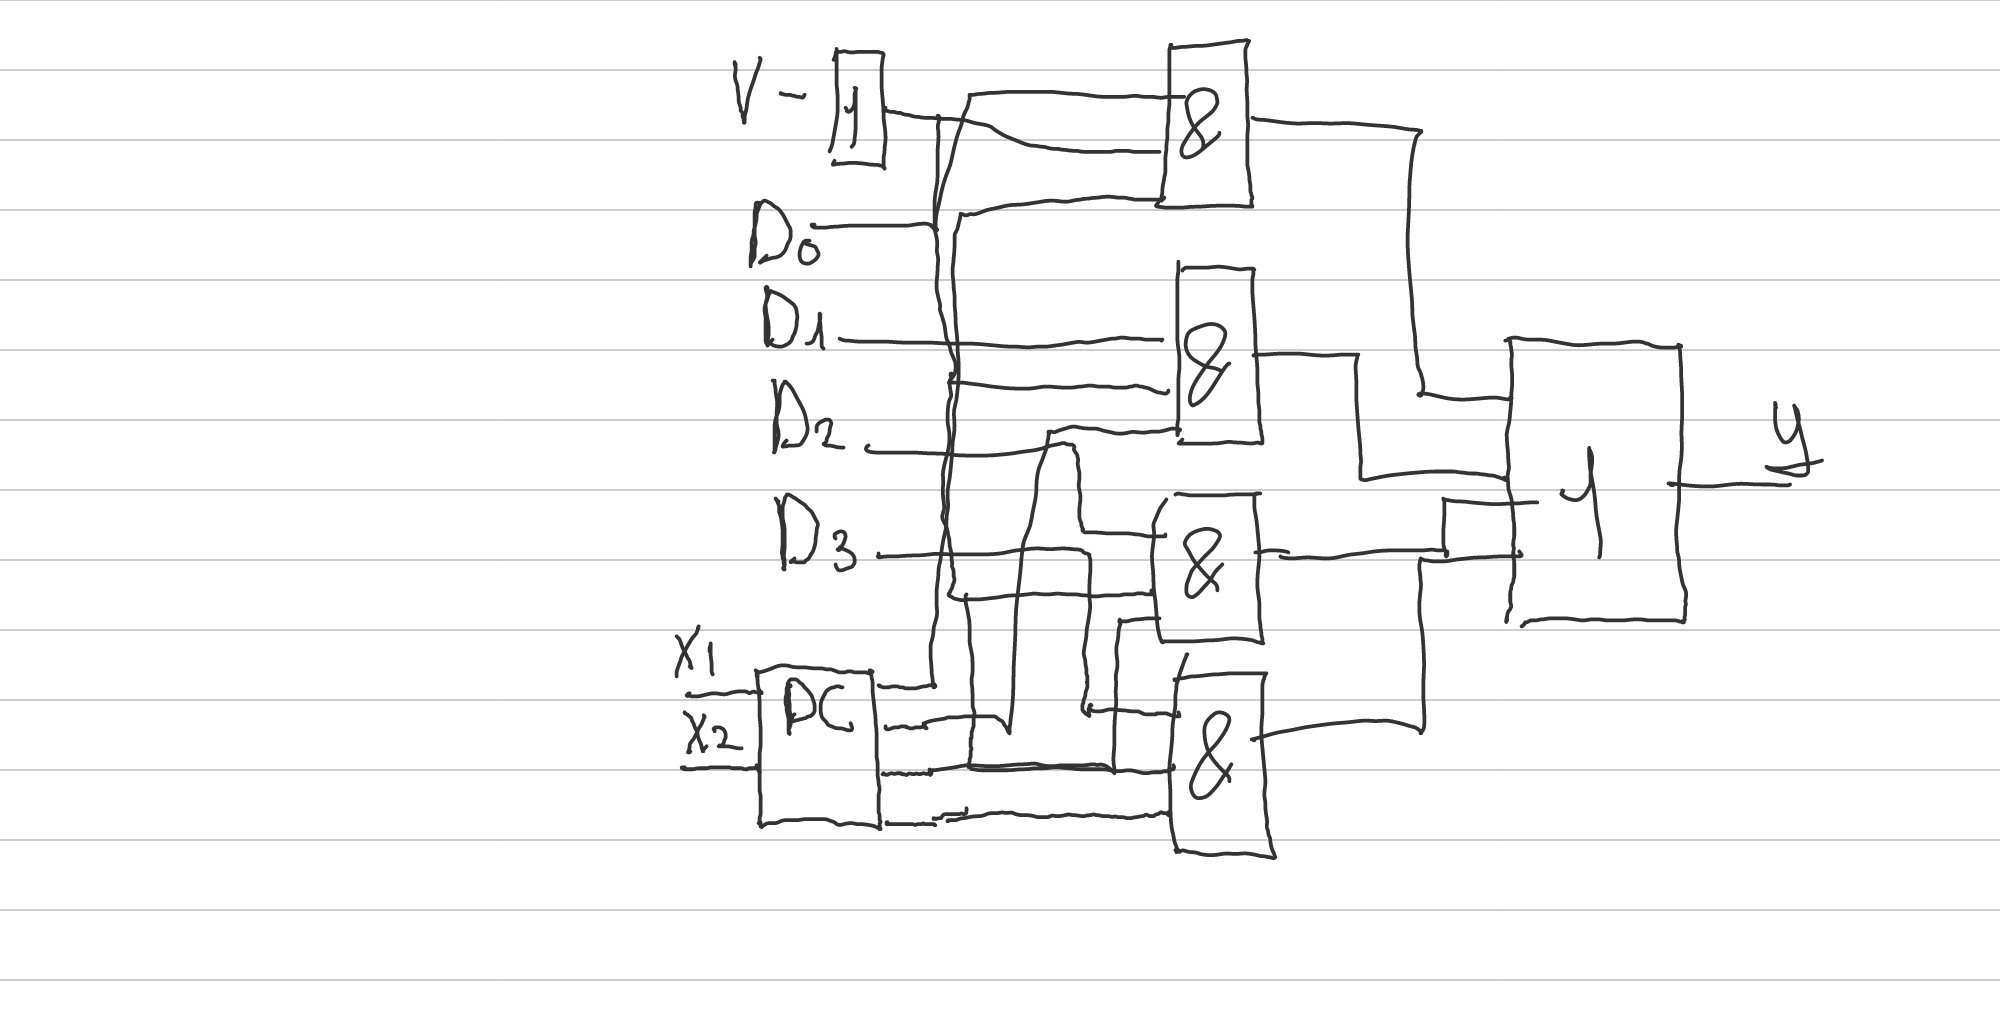
\includegraphics[width=\textwidth]{assets/multiplexer.png}

\subsubsection{Схема в multisim}

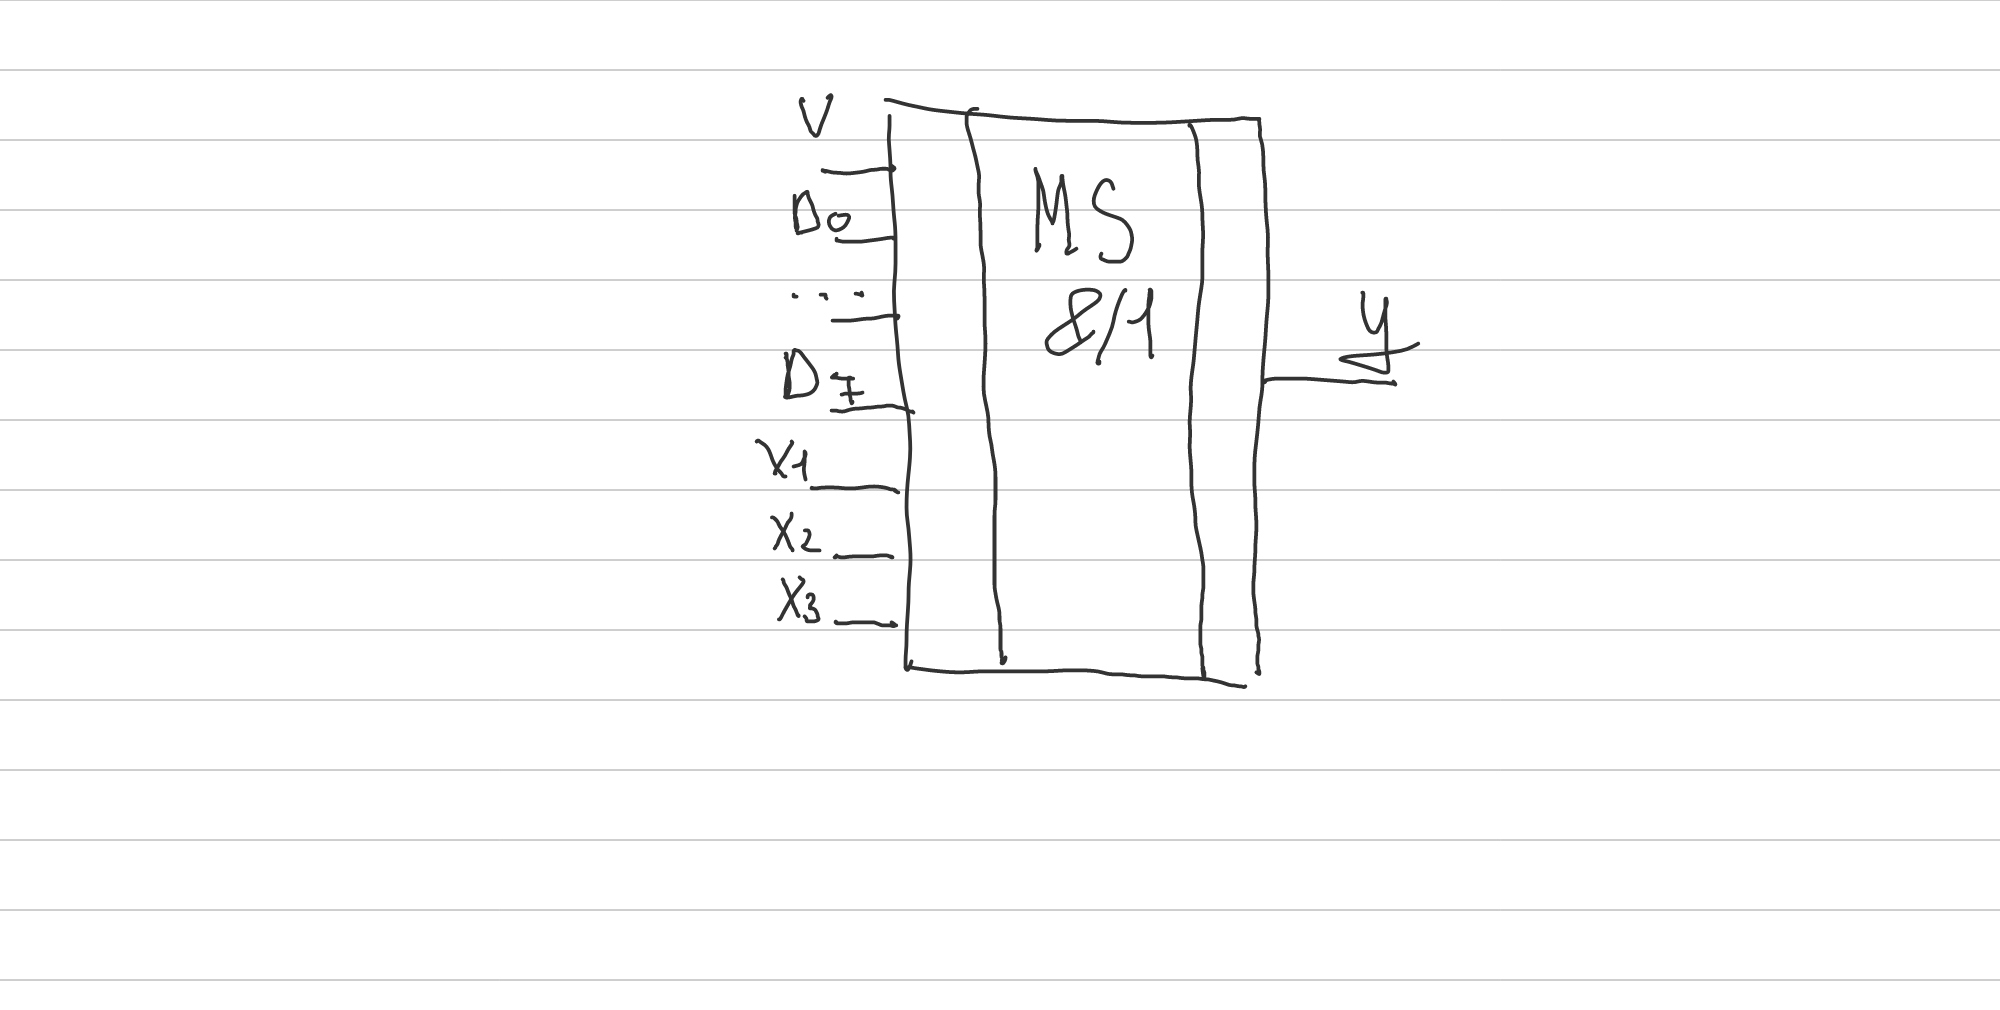
\includegraphics[width=\textwidth]{assets/multiplexer-multisim.png}

\subsection{Демультиплексор}

Демультиплексор — это логическое устройство, предназначенное для переключения сигнала с одного информационного входа на один из информационных выходов.

\hfill

Формула:

$y_0 = \overline{x_2} \overline{x_1} D, y_1 = \overline{x_1}D, y_2 = x_2\overline{x_1}D, y_3 = x_2 x_1 D$

\subsubsection{Схема}

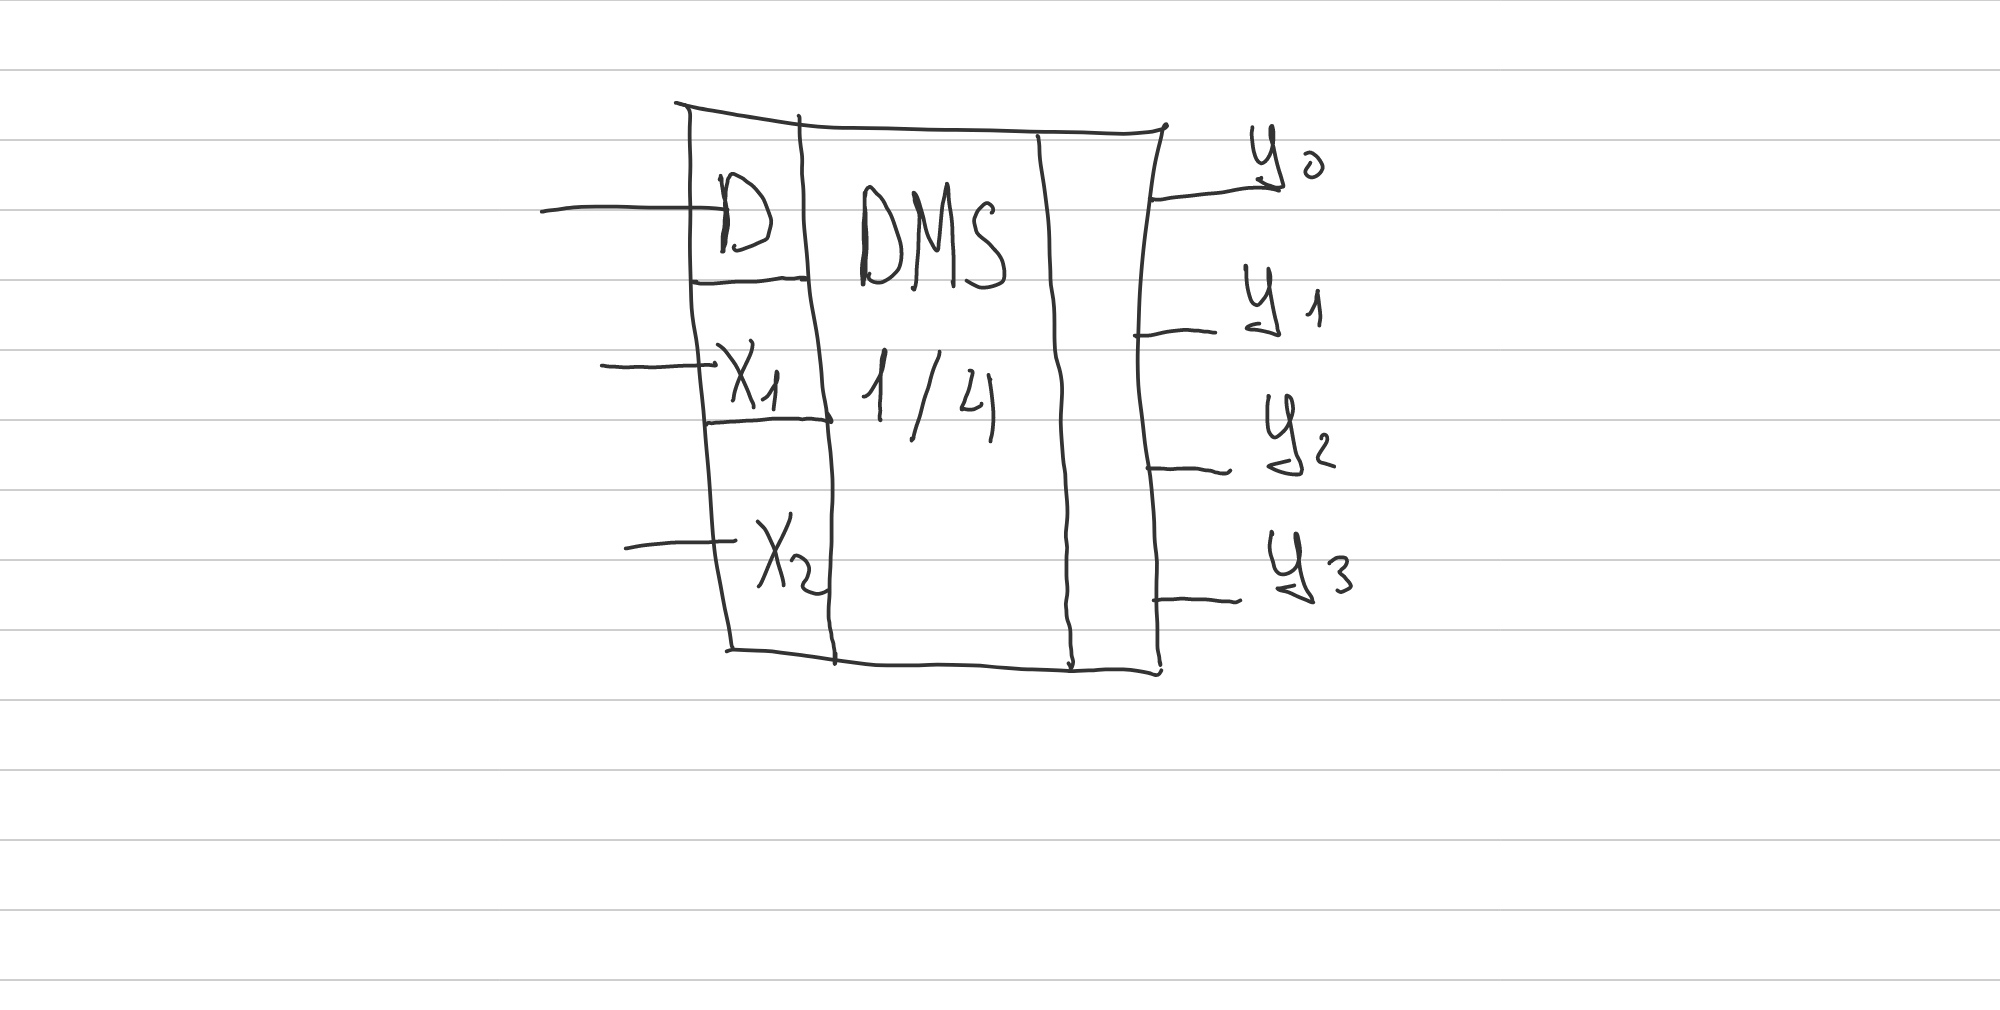
\includegraphics[width=\textwidth]{assets/demultiplexer.png}

\end{flushleft}

\end{document}